\documentclass[11pt]{article}
\RequirePackage[a4paper,top=2cm,left=2cm,right=2cm,bottom=3.5cm]{geometry}
\usepackage{booktabs}
\usepackage{enumerate}
\usepackage{biblatex} %Imports biblatex package
\addbibresource{bibliografia.bib} %Import the bibliography file
\setlength{\parindent}{0pt}
\usepackage[brazil]{babel}
\usepackage[utf8]{inputenc}
\usepackage{graphicx} 
\pagestyle{empty}
\usepackage{ragged2e}
\usepackage{amsmath}
\usepackage{listings}

%%%%%%%%%%%%%%%%%%%%%%%%%%%%%%%%%%%%%%%%%%%%%%%%%%%
% Macros de formatação Rodacki                    %
%%%%%%%%%%%%%%%%%%%%%%%%%%%%%%%%%%%%%%%%%%%%%%%%%%%
%\newcommand\commandname[number of arguments][value of optional argument]{code}
\newcommand{\bfit}[1]{\textbf{\textit{#1}}}

%%%%%%%%%%%%%%%%%%%%%%%%%%%%%%%%%%%%%%%%%%%%%%%%%%%
% Início                                          %
%%%%%%%%%%%%%%%%%%%%%%%%%%%%%%%%%%%%%%%%%%%%%%%%%%%

\begin{document}
\vspace{0.5cm}
\noindent

%%%%%%%%%%%%%%%%%%%%%%%%%%%%%%%%%%%%%%%%%%%%%%%%%%%
% Header                                          %
%%%%%%%%%%%%%%%%%%%%%%%%%%%%%%%%%%%%%%%%%%%%%%%%%%%    

\begin{minipage}{0.8\textwidth}
    \LARGE \textbf{Relatório do Trabalho Final}\\
    \Large Bacharelado em Ciência da Computação - Padrões de Projeto
    \Large Discentes: Matheus Marchi Moro e Celio Slomp
\end{minipage}

%%%%%%%%%%%%%%%%%%%%%%%%%%%%%%%%%%%%%%%%%%%%%%%%%%%
% Corpo do texto                                  %
%%%%%%%%%%%%%%%%%%%%%%%%%%%%%%%%%%%%%%%%%%%%%%%%%%% 
\pagenumbering{arabic}
\pagestyle {plain}
\vspace{0.5cm}
  
Este documento relata sobre um projeto de simulação de colisões que foi refeito utilizando os padrões de projeto \textit{Strategy} e \textit{Iterator}.

\vspace{0.5cm}
  
\section{Introdução}

\vspace{0.5cm}

O projeto original \cite{simulador_padroes} simula movimentação, aceleração e colisão entre corpos retangulares e circulares com algoritmos específicos para colidir círculo com círculo e círculo com retângulo \cite{colisao_circulo_circulo} \cite{colisao_circulo_retangulo}. Como a lógica de colisão é limitada devido ao fato de não utilizar um procedimento geral que se aplica a qualquer polígono, não foi possível otimizar esta parte específica com padrões de projeto. Contudo, pôde-se desacoplar tanto os diferentes comportamentos dos objetos que representam polígonos quanto a combinação de pares de polígonos para a verificação de colisão com os padrões \textit{Strategy} e \textit{Iterator} numa aplicação nova \cite{simulador_poo2}.

\section{Características do simulador}

O simulador inicial é um motor de colisões em duas dimensões escrito em \textit{C++} que utiliza a biblioteca \textit{Simple DirectMedia Layer 2} para visualização dos objetos e vetores matemáticos para o cálculo de física. \\

Sua estrutura é composta por uma classe \textit{App} que possui o laço principal do programa e duas listas de corpos que são submetidos à simulação. Esta classe utiliza as classes estáticas \textit{DisplayLogic} para desenhar as figuras na janela, \textit{MovementLogic} para mover os corpos e \textit{CollisionLogic} para verificar e tratar colisões. As listas de corpos, por usa vez, armazenam ponteiros para objetos RectBody ou CircleBody, respectivamente corpos retangulares e circulares. Desta forma, App itera sobre estas listas de corpos e os move, colide e mostra na tela, entre outros controles. O diagrama de classes está na figura~\ref{fig:diagr_original}. \\

\textbf{OBS.:} O diagrama da figura~\ref{fig:diagr_original} foi simplificado para fins de clareza. Desta forma, as variáveis de controle, o regulador de tempo, a classe que representa vetores bidimensionais e diversos métodos foram desprezados. Além disso, as classes estáticas \textit{Exhibition} e \textit{Mechanics} foram destrinchadas para \textit{DisplayLogic}, \textit{MovementLogic} e \textit{CollisionLogic} para se adequarem à compreensão do leitor.

 \begin{figure}[h]
    \centering
    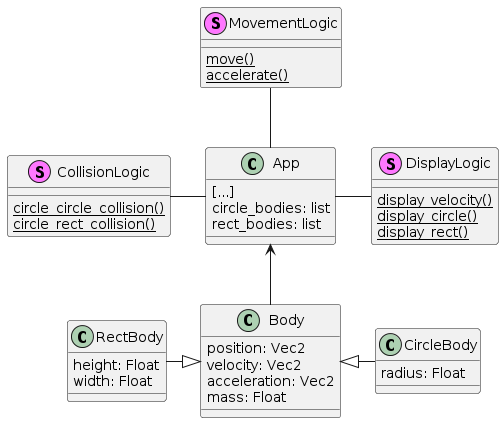
\includegraphics[scale=0.60]{figuras/diagr_original_simplificado.png}
    \caption{Diagrama de classes simplificado do simulador}
    \label{fig:diagr_original}
 \end{figure} 

\section{Problemas}

\subsection{Detecções de colisão}

Sejam $n$ corpos, App realiza $n^2 + n$ iterações para cada frame de simulação. São $n$ vezes para a movimentação e exibição dos corpos e $n^2$ vezes para as verificações de colisão. Como não houve a implementação de um algoritmo mais eficaz para estas verificações, foi necessário o uso de um algoritmo simples porém de ordem de complexidade $O(n^2)$ que escala mal. O número $n^2$ pode expressar uma matriz de iterações $A$, onde cada elemento $a_{ij}$ da matriz é um par $(b_i, b_j)$ de corpos.

$$A= 
\begin{bmatrix} (b_1, b_1) & (b_1, b_2) & \cdots & (b_1, b_j) \cr
(b_2, b_1) & (b_2, b_2) & \cdots & (b_2, b_j) \cr 
\vdots & \vdots & \ddots & \vdots \cr
(b_i, b_1) & (b_i, b_2) & \cdots & (b_i, b_j) \cr 
\end{bmatrix} $$ \\

Ao iterar sobre os elementos da matriz, \textit{App} efetua as seguintes operações:

\begin{itemize}
    \item Se $b_i = b_j$, continua para a próxima iteração pois não é possível colidir um corpo com ele mesmo. Neste caso, é toda a diagonal da matriz, ou seja, são $n$ iterações dispensadas;
    \item Se $b_i \neq b_j$, verifica se os corpos estão se aproximando. Caso estejam, verifica se um está sobrepondo o outro, isto é, se está ocorrendo uma colisão. Nesta condição, modifica os vetores de velocidade dos objetos. Aqui, é importante ressaltar que mesmo se os corpos estiverem se sobrepondo, não colidem se a distância entre eles tender ao aumento.
\end{itemize}

Entretanto, há um problema evidente neste método. Caso, por exemplo, a colisão $(b_1, b_2)$ seja apurada, posteriormente não vai ser necessário verificar a colisão $(b_2, b_1)$. O evento acontece também para $(b_1, b_3)$ e $(b_3, b_1)$, $(b_2, b_3)$ e $(b_3, b_2)$, e assim por diante. Em suma, para todo par $(b_m, b_n)$, a problemática acontece para $(b_n, b_m)$. Deste modo, todas as iterações inferiores à diagonal da matriz também são dispensadas, visto que não se precisa analisá-las. Portanto, a matriz de iterações efetiva $A'$ é a seguinte matriz, que será utilizada na refatoração:

$$A'= 
\begin{bmatrix} 0 & (b_1, b_2) & (b_1, b_3) & \cdots & (b_1, b_j) \cr
0 & 0 & (b_2, b_3) & \cdots & (b_2, b_j) \cr 
0 & 0 & 0 & \cdots & \vdots \cr 
\vdots & \vdots & \vdots & \ddots & (b_{i-1}, b_j) \cr
0 & 0 & \cdots & 0 & 0 \cr 
\end{bmatrix} $$ \\

\subsection{Acoplamento forte de representações de corpos}

Originalmente, decidiu-se representar somente retângulos e círculos nas simulações. Foi implementado o \textit{CircleBody} de maneira a ser visível, movimentar-se, acelerar e exibir vetor de velocidade. O \textit{RectBody}, por sua vez, não se move e nem exibe seu vetor de velocidade, mesmo o possuindo. Se o programador quisesse, neste caso, implementar um círculo que não se move, ele teria que criar uma classe nova e modificar a lógica de iterações dos corpos na \textit{App} criando uma lista específica para objetos desta classe. Caso deseje retângulos invisíveis que se movem, também deverá conceber outra classe diferente das demais e adicionar mais uma lista na \textit{App}. \\

Percebe-se então que os diferentes comportamentos dos polígonos estão fortemente acoplados no projeto, o  que gera manutenção desnecessária. Para somente duas representações, a implementação ainda não é tão trabalhosa. Entretanto, como é altamente provável que se queira simular diferentes polígonos e adicionar comportamentos num desenvolvimento futuro do simulador, viu-se a oportunidade de implementar o padrão de projeto Estratégia para resolução desta problemática.

\section{Refatoração}

\subsection{Principais mudanças}

Por questões de usabilidade e legibilidade, o projeto refatorado foi escrito em \textit{Python} e utilizou-se a biblioteca \textit{Pygame} com o mesmo intuito da \textit{Simple DirectMedia Layer 2}. Ademais, conforme o diagrama da figura~\ref{fig:diagr_refatorado}, adicionou-se ao projeto:

\begin{itemize}
    \item a interface \textit{Iterator} e sua classe concreta \textit{BodyIterator} que se relacionam ao padrão Iterador;
    \item as interfaces responsáveis pelo funcionamento do padrão Estratégia, que são \textit{MovementBehav}, \textit{VelDisplayBehav} e \textit{BodyDisplayBehav};
    \item um ponteiro \verb|body_iter| na \textit{App} para uma instância de \textit{BodyIterator};
    \item ponteiros em \textit{Body} para diferentes comportamentos de corpos, que são os atributos com final \verb|_behav|.
\end{itemize}

Além disso, por conta do Estratégia, foi possível eliminar as listas específicas de corpos em \textit{App} (\verb|circle_bodies| e \verb|rect_bodies|) e manter somente uma que armazena objetos \textit{Body} generalizados (\verb|bodies|). \\

A lógica da classe \textit{MovementLogic} foi incorporada na classe concreta de comportamento \textit{MovementBehav}. De maneira análoga, \textit{DisplayLogic} foi para as classes \textit{VelDisplayBehav} e \textit{BodyDisplayBehav}.

 \begin{figure}[h]
    \centering
    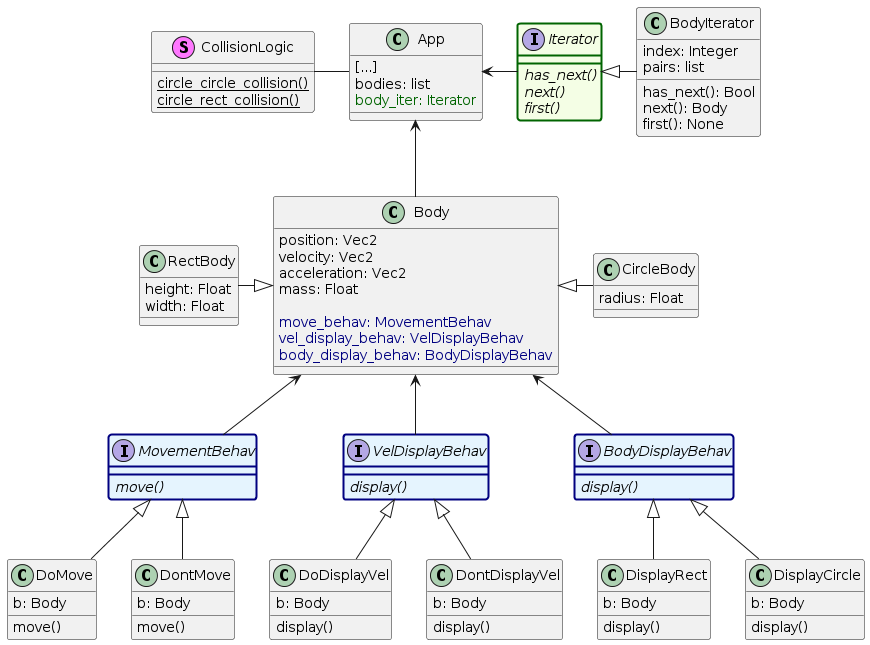
\includegraphics[scale=0.60]{figuras/diagr_refeito_simplificado.png}
    \caption{Diagrama de classes refatorado do simulador}
    \label{fig:diagr_refatorado}
 \end{figure} 

\subsection{Aplicação do padrão \textit{Iterator}}

Para o programa iterar sobre a matriz $A'$, foi utilizado o padrão Iterador para isto \cite{refac_guru_iter}. O Iterador Concreto, que é a classe \textit{BodyIterator}, foi implementada de modo a se especializar em oferecer um serviço de iteração mais efetivo para a verificação de colisões dos corpos. Esta classe recebe a lista de corpos de \textit{App}, representada pela matriz $A$, monta internamente uma lista dos pares especificados na matriz $A'$, armazena um índice atual \textit{index} e oferece métodos de iteração sobre esta lista. A lista dos pares tem o nome \verb|pairs| e os métodos são \verb|has_next()|, \verb|next()| e \verb|first()|. Não foi utilizada uma classe \textit{ConcreteCollection} pois a estrutura \verb|pairs| é simples demais para necessitar gestão própria. \\

O tipo de lista utilizado em todo o projeto foi o tipo primitivo \verb|list| do Python. Este tipo de lista é armazenado como um array na memória e possui um acesso de tempo constante \cite{time_complexity}, o que não contradiz a próxima constatação: desprezando o tempo de acesso à lista \verb|pairs|, já que é constante, o algoritmo que a itera tem ordem de complexidade $O(\frac{n^2 - n}{2})$, que é aproximadamente 100\% melhor que o algoritmo anterior. Percebe-se que, nesta ordem de complexidade, $n^2$ representa toda a matriz $A$, enquanto que $n$ é sua diagonal e a fração $1/2$, ao multiplicar $n^2$ e $n$, corresponde à sua matriz triangular inferior. O número
$$\frac{n^2 - n}{2}$$
oferece a quantidade de elementos da lista que é utilizada pelo método \verb|has_next()|. Curiosamente, também é possível obter esta quantidade ao calcular 
$$\frac{n!}{2!(n-2)!}$$
que é a combinação simples de todos os corpos tomados de 2 em 2. \\

Os métodos desta classe são caracterizados a seguir.

\begin{itemize}
    \item \verb|has_next()|: Retorna um valor booleano \textit{True} se a lista ainda possui elementos a serem iterados. Caso esteja no último elemento, retorna \textit{False};
    \item \verb|next()|: Retorna o atual par de corpos $(bi, bj)$ na forma de tupla e incrementa \verb|index| em 1;
    \item \verb|first()|: Faz com que \verb|index| receba o valor 0.
\end{itemize}

Com esses três métodos e a lógica de concepção da lista \verb|pairs| embutida no construtor da classe, é possível utilizar a mesma estrutura várias vezes sem precisar recriá-la. \textit{App} então usa os pares retornados pelo método \verb|next()| e os passa como parâmetros diretamente aos métodos da classe \textit{CollisionLogic} após uma verificação de tipos, sem precisar de uma implementação \textit{hard code} para gerir as iterações.

\subsection{Aplicação do padrão \textit{Strategy}}

Usufruiu-se do padrão de projeto Estratégia \cite{refac_guru_strategy} para desacoplar as diferentes particularidades dos corpos e oferecer uma gestão dinâmica de suas características. Ao criar os atributos com fim \verb|_behav| na classe \textit{Body} que apontam para comportamentos concretos, possibilitou-se também a escalabilidade do projeto, visto que para alterar os procederes dos corpos basta mudar as instâncias de comportamentos antes do laço principal. E, para adicionar, é suficiente criar novos comportamentos concretos e/ou acrescentar ponteiros na \textit{Body}. Tudo isto sem precisar de modificações na \textit{App}. \\

Não obstante, o projeto original contém uma classe chamada \textit{Persistance} que carrega as listas de corpos e armazena os resultados da simulação. Por conta do \textit{Strategy}, tornou-se possível a leitura de diferentes peculiaridades dos corpos a partir de um \textit{input}, ou arquivo, o que estabelece uma simulação mais personalizável. \\

Os métodos das classes concretas são detalhados a seguir.

\begin{itemize}
    \item \textit{MovementBehav}, método \verb|move()|
    \begin{itemize}
        \item \textit{DoMove}: Adiciona a velocidade à posição do corpo e depois adiciona a aceleração à velocidade do corpo. Ou seja, faz basicamente
            \begin{lstlisting}[language=Python]
                b.position = b.position + b.velocity
                b.velocity = b.velocity + b.acceleration
            \end{lstlisting}
        onde \verb|b| é o ponteiro do corpo, \verb|position| é o vetor de posição, \verb|velocity| é o vetor de velocidade e \verb|acceleration| é o vetor de aceleração. A classe \textit{Vec2}, responsável pela administração dos vetores matemáticos, já faz a sobrecarga do operador de soma;
        \item \textit{DontMove}: Executa \verb|pass| \cite{pass}. Este comando faz nada;
    \end{itemize}

    \item \textit{VelDisplayBehav}, método \verb|display()|
    \begin{itemize}
        \item \textit{DoDisplayVel}: Exibe o vetor de velocidade do objeto. Pinta uma reta na tela a partir da posição do corpo até a posição + velocidade e depois a completa com retas menores para formar a ponta da flecha;
        \item \textit{DontDisplayVel}: Faz nada. Não mostra o vetor;
    \end{itemize}
    
    \item \textit{BodyDisplayBehav}, método \verb|display()|
    \begin{itemize}
        \item \textit{DisplayRect}: Desenha quatro retas na tela de modo a formarem o retângulo. Utiliza a posição do objeto, sua altura e sua largura;
        \item \textit{DisplayCircle}: Divide uma circuferência em uma quantidade $x$ de fatias para deduzir o ângulo $\alpha$ entre cada secção em radianos. Ou seja, uma circunferência desenhada com este algoritmo tem $x$ lados. O número escolhido no projeto foi $18$ pois é uma quantidade confortável de lados e não muito custosa. Após isso, o algoritmo cria dois vetores, rotaciona um deles em $\alpha$ radianos e depois desenha uma reta de um vetor a outro e rotaciona ambos $x$ vezes, até completar a circunferência;
        \item (IMPLEMENTADO EM AMBIENTE DE TESTES) \textit{DisplayNothing}: Faz nada (corpo invisível).
    \end{itemize}
\end{itemize}

\printbibliography %Prints bibliography
	
\end{document}
